\begin{minipage}[t]{180mm}
\fcolorbox{black}{white}{
\begin{minipage}[b]{30mm}

\includegraphics[width=0.5\linewidth]{unflogo.pdf}
\end{minipage}
\begin{minipage}[b]{100mm}
\Huge \textbf{UNF NEWZ} \\
\Large -- Søvn og retsstavning er overvurderet! 
\end{minipage}
\begin{minipage}[b]{50mm}
\Large Onsdag 17.07.2015 \\
\normalsize Redigeret i \LaTeX\ af \\ SOM, MGS, MMN, SABH
\end{minipage}
}
\end{minipage}



\begin{minipage}[b]{0.95\linewidth}
\begin{minipage}[t]{0.47\textwidth}
\vspace{3mm}
\section*{Produktanmeldelse -- Internettet}
Ved første øjenkast ses straks at her er der kræset for detaljerne. Siden 1980'erne har internettet været et vigtigt hjælpemiddel i videnskabelige diskussioner og kulturel diskurs. I 1990'erne udviklede det sig til ensomme unges primære fritidsaktivitet og verdensøkonomiens største uprodiktive bobbel. I 2000'erne har det  udviklet sig til det primære opholdssted for nuttede dyr og nøgne mennesker, og har derved fået en altomfattende betydning for civiliserede menneskers kulturelle dannelse, som erstatning for beskadigede mineraler og tynde stykker træ, som ungdommen end ikke kan huske. I 2010'erne erstatettede internettet menneskelig kontakt og faglige kvalifikationer blev erstattet af opadpegende tommelfingre, og kulturkanonen af dårlige videoptagelser af kartoffelkanoner. Derpå, i 2020'erne endte internettet med at dokumenterede verden, og verden begyndte at dokumentere internettet, indtil den 29. oktober 2019, hvor en troll slettede den svage vekselvirkning fra den førende kinesiske wiki, hvilke resulterede i, at alle atomer i universet spontan henfaldt, og dermed afsluttede universets og muligvis internettets eksistens, men samtidigt bekræftede flere af de førende konspirationsteorier.Internettet indeholdt små katte og dårlige jokes og er derfor ikke egnet til voksne over 30 år.

\vspace{1mm}
\section*{Williams paradox}
Jeg kan godt li' folk der står op.

\vspace{1mm}
\section*{Dagens sætning om $3$}
\begin{align*}
3 &= \sqrt{1+2\sqrt{1+3\sqrt{1+4\sqrt{1+5\sqrt{1+}\dots}}}}
\end{align*}

\vspace{1mm}
\section*{Madanmeldelse -- Helstegt spædbarn}
\fcolorbox{black}{white}{$13$ ud af $\aleph_2$ chokoladekiks}

\vspace{2mm}
Som led i grevskabet Thalias festmiddag i går aftes fik jeg langt om længe igen mulighed for at spise helstegt spædbarn. Det var en fornøjelse af dimensioner for en conniseur som mig. Desværre har der nemlig i de sidste år været en uheldig udvikling i det østjydske kanibal-restaurantsmiljø. Af mig uforklarlige grunde går trenden mod finthakkede indre organer stegt med asiatiske krydderier. Dette smager måske godt de første par gange, og er lidt lettere tilgængeligt for uerfarne kokke, men man taber smagen af sprødstegt nyfødt hud og kogte usvækkede øjne. Også nogle af de indre organger, specielt de som spædbørn endnnu ikke har behov for, og som derfor stadig er friske og ubrugte og som i dette tilfælde var bloddryppende og kun let gennemstegt på den gode måde. Eneste kritik på denne festmiddag er, at forretten ikke var helt tilfredsstillende, da nogle af hjernerne ikke virker til at komme fra synderligt intelligente eksdeltagere.

\end{minipage}%
\hfill\begin{minipage}[t]{0.47\textwidth}
\vspace{3mm}
\section*{Vejrudsigt}
\textbf{IMF, AU (fra DMI)}: Skyet med ingen regn og vind fra vest. Op til 20 grader om dagen og ned til 12 grader om natten.

\textbf{JAM}: 3 til 6 grader med svag vind fra nordvest og høj sol. Risiko for isbjørneangreb.

\vspace{-2mm}
\section*{Dagens mediciner}
Hvis du møder en mediciner, så prik hende, og forklar stilfærdig, at håndspålægning er den eneste behandling, du tror på.

\vspace{-2mm}
\section*{Find en Fynbo}
Under dække af dværgenes angreb, har Fynboen sneget sig ind i dagens avis igen, find ham og smadder hans knæ.

\vspace{-2mm}
\section*{Fakta om Jylland}
Jyder er chill, fordi de kan komme længere nordpå end andre danskere, uden at komme udenfor deres comfort zone

\vspace{-2mm}
\section*{Dagens sandsynlighed}
Sandsynligheden for at en hundværg har skæg er $1$.

\vspace{1mm}
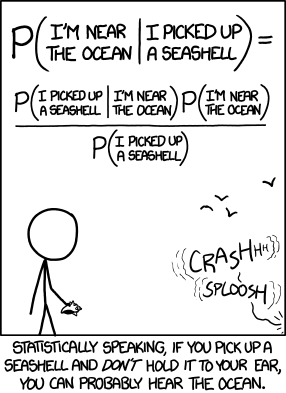
\includegraphics[width=95mm]{seashell.png}
\tiny Randall Munroe, http://xkcd.com/1236/, CC-BY-SA-2.5
\end{minipage}

\begin{center}
\tiny UNF Newz er avisen hvor at ansvarshavende redaktør fralægger sig ethvert ansvar for eventuel plagiering, kaniner, tysk, stavefelj, kaffe, dårlig humor, glemsomhed, katte, store sigmaer, pile, skyer, dårlige oversættelser og alt hvad eventuelle homo sapiens sapiens kunne finde på at holde imod UNF Newz! Dog tager UNF Newz fuld credit og copyright for alle guldkorn, magickort, mus, \TeX, humor, smil, Mortener, kaffe, før-fremtid, ringe og/eller rubik's cube.
\end{center}
\end{minipage}

